% Figure from MATH 591 notes, section 65 (Lecture 22): exhaustion function and slicing.
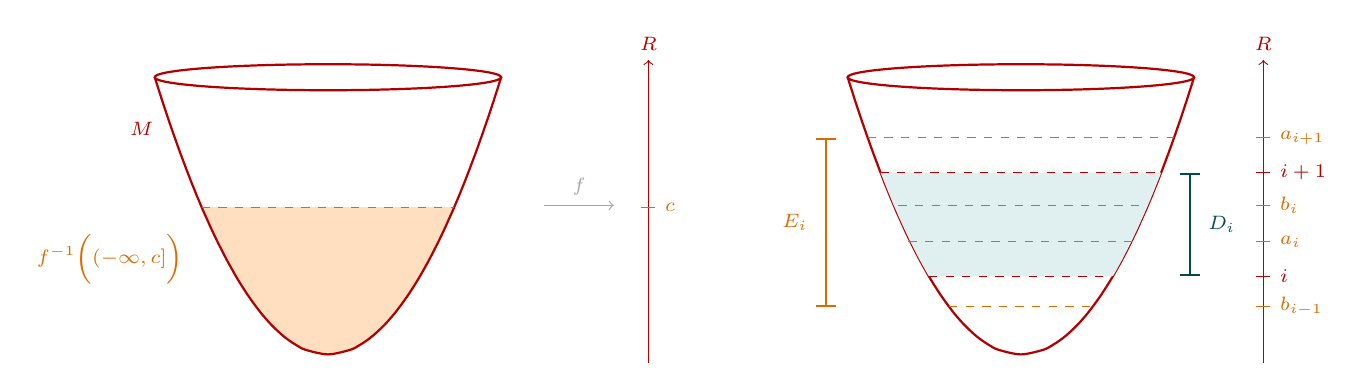
\begin{tikzpicture}[scale=1.1]
\fill[orange!25] plot coordinates {(-1.458,1.700) (-1.439,1.657) (-1.421,1.615) (-1.402,1.573) (-1.383,1.530) (-1.364,1.488) (-1.344,1.445) (-1.324,1.402) (-1.304,1.360) (-1.283,1.317) (-1.262,1.275) (-1.241,1.232) (-1.220,1.190) (-1.198,1.147) (-1.175,1.105) (-1.152,1.062) (-1.129,1.020) (-1.105,0.978) (-1.081,0.935) (-1.056,0.893) (-1.031,0.850) (-1.005,0.808) (-0.978,0.765) (-0.950,0.722) (-0.922,0.680) (-0.893,0.637) (-0.862,0.595) (-0.831,0.552) (-0.798,0.510) (-0.764,0.468) (-0.729,0.425) (-0.691,0.383) (-0.652,0.340) (-0.610,0.297) (-0.565,0.255) (-0.515,0.212) (-0.461,0.170) (-0.399,0.127) (-0.326,0.085) (-0.230,0.042) (-0.000,0.000) (0.230,0.042) (0.326,0.085) (0.399,0.128) (0.461,0.170) (0.515,0.212) (0.565,0.255) (0.610,0.297) (0.652,0.340) (0.691,0.382) (0.729,0.425) (0.764,0.467) (0.798,0.510) (0.831,0.552) (0.862,0.595) (0.893,0.637) (0.922,0.680) (0.950,0.722) (0.978,0.765) (1.005,0.807) (1.031,0.850) (1.056,0.892) (1.081,0.935) (1.105,0.978) (1.129,1.020) (1.152,1.062) (1.175,1.105) (1.198,1.147) (1.220,1.190) (1.241,1.232) (1.262,1.275) (1.283,1.317) (1.304,1.360) (1.324,1.403) (1.344,1.445) (1.364,1.488) (1.383,1.530) (1.402,1.573) (1.421,1.615) (1.439,1.657) (1.458,1.700)} -- cycle;
\draw[red!70!black, thick] plot[smooth] coordinates {(-2.000,3.200) (-1.983,3.147) (-1.966,3.093) (-1.949,3.040) (-1.932,2.987) (-1.915,2.933) (-1.897,2.880) (-1.880,2.827) (-1.862,2.773) (-1.844,2.720) (-1.826,2.667) (-1.807,2.613) (-1.789,2.560) (-1.770,2.507) (-1.751,2.453) (-1.732,2.400) (-1.713,2.347) (-1.693,2.293) (-1.673,2.240) (-1.653,2.187) (-1.633,2.133) (-1.612,2.080) (-1.592,2.027) (-1.571,1.973) (-1.549,1.920) (-1.528,1.867) (-1.506,1.813) (-1.483,1.760) (-1.461,1.707) (-1.438,1.653) (-1.414,1.600) (-1.390,1.547) (-1.366,1.493) (-1.342,1.440) (-1.317,1.387) (-1.291,1.333) (-1.265,1.280) (-1.238,1.227) (-1.211,1.173) (-1.183,1.120) (-1.155,1.067) (-1.125,1.013) (-1.095,0.960) (-1.065,0.907) (-1.033,0.853) (-1.000,0.800) (-0.966,0.747) (-0.931,0.693) (-0.894,0.640) (-0.856,0.587) (-0.816,0.533) (-0.775,0.480) (-0.730,0.427) (-0.683,0.373) (-0.632,0.320) (-0.577,0.267) (-0.516,0.213) (-0.447,0.160) (-0.365,0.107) (-0.258,0.053) (0.000,0.000) (0.258,0.053) (0.365,0.107) (0.447,0.160) (0.516,0.213) (0.577,0.267) (0.632,0.320) (0.683,0.373) (0.730,0.427) (0.775,0.480) (0.816,0.533) (0.856,0.587) (0.894,0.640) (0.931,0.693) (0.966,0.747) (1.000,0.800) (1.033,0.853) (1.065,0.907) (1.095,0.960) (1.125,1.013) (1.155,1.067) (1.183,1.120) (1.211,1.173) (1.238,1.227) (1.265,1.280) (1.291,1.333) (1.317,1.387) (1.342,1.440) (1.366,1.493) (1.390,1.547) (1.414,1.600) (1.438,1.653) (1.461,1.707) (1.483,1.760) (1.506,1.813) (1.528,1.867) (1.549,1.920) (1.571,1.973) (1.592,2.027) (1.612,2.080) (1.633,2.133) (1.653,2.187) (1.673,2.240) (1.693,2.293) (1.713,2.347) (1.732,2.400) (1.751,2.453) (1.770,2.507) (1.789,2.560) (1.807,2.613) (1.826,2.667) (1.844,2.720) (1.862,2.773) (1.880,2.827) (1.897,2.880) (1.915,2.933) (1.932,2.987) (1.949,3.040) (1.966,3.093) (1.983,3.147) (2.000,3.200)};
\draw[red!70!black, thick] (0,3.2) ellipse (2.000 and 0.15);
\draw[orange!85!black, dashed] (-1.458,1.7) -- (1.458,1.7);
\node[orange!85!black, font=\scriptsize, anchor=east] at (-1.558,1.100) {$f^{-1}\big((-\infty, c]\big)$};
\draw[->, gray!70] (2.5,1.72) -- node[above, font=\scriptsize] {$f$} (3.3,1.72);
\draw[->, red!70!black] (3.7,-0.1) -- (3.7,3.4) node[above, font=\scriptsize] {$\mathbb{R}$};
\draw[orange!85!black] (3.62,1.7) -- (3.78,1.7) node[right, font=\scriptsize] {$c$};
\node[red!70!black, font=\scriptsize] at (-2.15,2.6) {$M$};
\draw[red!70!black, thick] plot[smooth] coordinates {(6.000,3.200) (6.017,3.147) (6.034,3.093) (6.051,3.040) (6.068,2.987) (6.085,2.933) (6.103,2.880) (6.120,2.827) (6.138,2.773) (6.156,2.720) (6.174,2.667) (6.193,2.613) (6.211,2.560) (6.230,2.507) (6.249,2.453) (6.268,2.400) (6.287,2.347) (6.307,2.293) (6.327,2.240) (6.347,2.187) (6.367,2.133) (6.388,2.080) (6.408,2.027) (6.429,1.973) (6.451,1.920) (6.472,1.867) (6.494,1.813) (6.517,1.760) (6.539,1.707) (6.562,1.653) (6.586,1.600) (6.610,1.547) (6.634,1.493) (6.658,1.440) (6.683,1.387) (6.709,1.333) (6.735,1.280) (6.762,1.227) (6.789,1.173) (6.817,1.120) (6.845,1.067) (6.875,1.013) (6.905,0.960) (6.935,0.907) (6.967,0.853) (7.000,0.800) (7.034,0.747) (7.069,0.693) (7.106,0.640) (7.144,0.587) (7.184,0.533) (7.225,0.480) (7.270,0.427) (7.317,0.373) (7.368,0.320) (7.423,0.267) (7.484,0.213) (7.553,0.160) (7.635,0.107) (7.742,0.053) (8.000,0.000) (8.258,0.053) (8.365,0.107) (8.447,0.160) (8.516,0.213) (8.577,0.267) (8.632,0.320) (8.683,0.373) (8.730,0.427) (8.775,0.480) (8.816,0.533) (8.856,0.587) (8.894,0.640) (8.931,0.693) (8.966,0.747) (9.000,0.800) (9.033,0.853) (9.065,0.907) (9.095,0.960) (9.125,1.013) (9.155,1.067) (9.183,1.120) (9.211,1.173) (9.238,1.227) (9.265,1.280) (9.291,1.333) (9.317,1.387) (9.342,1.440) (9.366,1.493) (9.390,1.547) (9.414,1.600) (9.438,1.653) (9.461,1.707) (9.483,1.760) (9.506,1.813) (9.528,1.867) (9.549,1.920) (9.571,1.973) (9.592,2.027) (9.612,2.080) (9.633,2.133) (9.653,2.187) (9.673,2.240) (9.693,2.293) (9.713,2.347) (9.732,2.400) (9.751,2.453) (9.770,2.507) (9.789,2.560) (9.807,2.613) (9.826,2.667) (9.844,2.720) (9.862,2.773) (9.880,2.827) (9.897,2.880) (9.915,2.933) (9.932,2.987) (9.949,3.040) (9.966,3.093) (9.983,3.147) (10.000,3.200)};
\draw[red!70!black, thick] (8.000,3.2) ellipse (2.000 and 0.15);
\fill[teal!12] plot coordinates {(6.380,2.100) (6.395,2.060) (6.411,2.020) (6.427,1.980) (6.443,1.940) (6.459,1.900) (6.475,1.860) (6.492,1.820) (6.508,1.780) (6.525,1.740) (6.542,1.700) (6.560,1.660) (6.577,1.620) (6.595,1.580) (6.613,1.540) (6.631,1.500) (6.649,1.460) (6.668,1.420) (6.687,1.380) (6.706,1.340) (6.725,1.300) (6.745,1.260) (6.765,1.220) (6.786,1.180) (6.806,1.140) (6.827,1.100) (6.849,1.060) (6.871,1.020) (6.893,0.980) (6.916,0.940) (6.939,0.900) (9.061,0.900) (9.084,0.940) (9.107,0.980) (9.129,1.020) (9.151,1.060) (9.173,1.100) (9.194,1.140) (9.214,1.180) (9.235,1.220) (9.255,1.260) (9.275,1.300) (9.294,1.340) (9.313,1.380) (9.332,1.420) (9.351,1.460) (9.369,1.500) (9.387,1.540) (9.405,1.580) (9.423,1.620) (9.440,1.660) (9.458,1.700) (9.475,1.740) (9.492,1.780) (9.508,1.820) (9.525,1.860) (9.541,1.900) (9.557,1.940) (9.573,1.980) (9.589,2.020) (9.605,2.060) (9.620,2.100)} -- cycle;
\draw[->, red!70!black] (10.800,-0.1) -- (10.800,3.4) node[above, font=\scriptsize] {$\mathbb{R}$};
\draw[orange!85!black, dashed] (7.171,0.55) -- (8.829,0.55);
\draw[orange!85!black] (10.720,0.55) -- (10.880,0.55) node[right, font=\scriptsize] {$b_{i-1}$};
\draw[red!70!black, dashed] (6.939,0.9) -- (9.061,0.9);
\draw[red!70!black] (10.720,0.9) -- (10.880,0.9) node[right, font=\scriptsize] {$i$};
\draw[orange!85!black, dashed] (6.701,1.3) -- (9.299,1.3);
\draw[orange!85!black] (10.720,1.3) -- (10.880,1.3) node[right, font=\scriptsize] {$a_i$};
\draw[orange!85!black, dashed] (6.586,1.72) -- (9.414,1.72);
\draw[orange!85!black] (10.720,1.72) -- (10.880,1.72) node[right, font=\scriptsize] {$b_i$};
\draw[red!70!black, dashed] (6.380,2.1) -- (9.620,2.1);
\draw[red!70!black] (10.720,2.1) -- (10.880,2.1) node[right, font=\scriptsize] {$i+1$};
\draw[orange!85!black, dashed] (6.232,2.5) -- (9.768,2.5);
\draw[orange!85!black] (10.720,2.5) -- (10.880,2.5) node[right, font=\scriptsize] {$a_{i+1}$};
\draw[thick, orange!85!black, |-|] (5.750,0.55) -- (5.750,2.5) node[midway, left=3pt, font=\scriptsize] {$E_i$};
\draw[thick, teal!60!black, |-|] (9.950,0.9) -- (9.950,2.1) node[midway, right=3pt, font=\scriptsize] {$D_i$};
\end{tikzpicture}
